\documentclass[11pt,preprint, authoryear]{elsarticle}

\usepackage{lmodern}
%%%% My spacing
\usepackage{setspace}
\setstretch{1.2}
\DeclareMathSizes{12}{14}{10}{10}

% Wrap around which gives all figures included the [H] command, or places it "here". This can be tedious to code in Rmarkdown.
\usepackage{float}
\let\origfigure\figure
\let\endorigfigure\endfigure
\renewenvironment{figure}[1][2] {
    \expandafter\origfigure\expandafter[H]
} {
    \endorigfigure
}

\let\origtable\table
\let\endorigtable\endtable
\renewenvironment{table}[1][2] {
    \expandafter\origtable\expandafter[H]
} {
    \endorigtable
}


\usepackage{ifxetex,ifluatex}
\usepackage{fixltx2e} % provides \textsubscript
\ifnum 0\ifxetex 1\fi\ifluatex 1\fi=0 % if pdftex
  \usepackage[T1]{fontenc}
  \usepackage[utf8]{inputenc}
\else % if luatex or xelatex
  \ifxetex
    \usepackage{mathspec}
    \usepackage{xltxtra,xunicode}
  \else
    \usepackage{fontspec}
  \fi
  \defaultfontfeatures{Mapping=tex-text,Scale=MatchLowercase}
  \newcommand{\euro}{€}
\fi

\usepackage{amssymb, amsmath, amsthm, amsfonts}

\def\bibsection{\section*{References}} %%% Make "References" appear before bibliography


\usepackage[round]{natbib}

\usepackage{longtable}
\usepackage[margin=2.3cm,bottom=2cm,top=2.5cm, includefoot]{geometry}
\usepackage{fancyhdr}
\usepackage[bottom, hang, flushmargin]{footmisc}
\usepackage{graphicx}
\numberwithin{equation}{section}
\numberwithin{figure}{section}
\numberwithin{table}{section}
\setlength{\parindent}{0cm}
\setlength{\parskip}{1.3ex plus 0.5ex minus 0.3ex}
\usepackage{textcomp}
\renewcommand{\headrulewidth}{0.2pt}
\renewcommand{\footrulewidth}{0.3pt}

\usepackage{array}
\newcolumntype{x}[1]{>{\centering\arraybackslash\hspace{0pt}}p{#1}}

%%%%  Remove the "preprint submitted to" part. Don't worry about this either, it just looks better without it:
\makeatletter
\def\ps@pprintTitle{%
  \let\@oddhead\@empty
  \let\@evenhead\@empty
  \let\@oddfoot\@empty
  \let\@evenfoot\@oddfoot
}
\makeatother

 \def\tightlist{} % This allows for subbullets!

\usepackage{hyperref}
\hypersetup{breaklinks=true,
            bookmarks=true,
            colorlinks=true,
            citecolor=blue,
            urlcolor=blue,
            linkcolor=blue,
            pdfborder={0 0 0}}


% The following packages allow huxtable to work:
\usepackage{siunitx}
\usepackage{multirow}
\usepackage{hhline}
\usepackage{calc}
\usepackage{tabularx}
\usepackage{booktabs}
\usepackage{caption}


\newenvironment{columns}[1][]{}{}

\newenvironment{column}[1]{\begin{minipage}{#1}\ignorespaces}{%
\end{minipage}
\ifhmode\unskip\fi
\aftergroup\useignorespacesandallpars}

\def\useignorespacesandallpars#1\ignorespaces\fi{%
#1\fi\ignorespacesandallpars}

\makeatletter
\def\ignorespacesandallpars{%
  \@ifnextchar\par
    {\expandafter\ignorespacesandallpars\@gobble}%
    {}%
}
\makeatother

\newlength{\cslhangindent}
\setlength{\cslhangindent}{1.5em}
\newenvironment{CSLReferences}%
  {\setlength{\parindent}{0pt}%
  \everypar{\setlength{\hangindent}{\cslhangindent}}\ignorespaces}%
  {\par}


\urlstyle{same}  % don't use monospace font for urls
\setlength{\parindent}{0pt}
\setlength{\parskip}{6pt plus 2pt minus 1pt}
\setlength{\emergencystretch}{3em}  % prevent overfull lines
\setcounter{secnumdepth}{5}

%%% Use protect on footnotes to avoid problems with footnotes in titles
\let\rmarkdownfootnote\footnote%
\def\footnote{\protect\rmarkdownfootnote}
\IfFileExists{upquote.sty}{\usepackage{upquote}}{}

%%% Include extra packages specified by user

%%% Hard setting column skips for reports - this ensures greater consistency and control over the length settings in the document.
%% page layout
%% paragraphs
\setlength{\baselineskip}{12pt plus 0pt minus 0pt}
\setlength{\parskip}{12pt plus 0pt minus 0pt}
\setlength{\parindent}{0pt plus 0pt minus 0pt}
%% floats
\setlength{\floatsep}{12pt plus 0 pt minus 0pt}
\setlength{\textfloatsep}{20pt plus 0pt minus 0pt}
\setlength{\intextsep}{14pt plus 0pt minus 0pt}
\setlength{\dbltextfloatsep}{20pt plus 0pt minus 0pt}
\setlength{\dblfloatsep}{14pt plus 0pt minus 0pt}
%% maths
\setlength{\abovedisplayskip}{12pt plus 0pt minus 0pt}
\setlength{\belowdisplayskip}{12pt plus 0pt minus 0pt}
%% lists
\setlength{\topsep}{10pt plus 0pt minus 0pt}
\setlength{\partopsep}{3pt plus 0pt minus 0pt}
\setlength{\itemsep}{5pt plus 0pt minus 0pt}
\setlength{\labelsep}{8mm plus 0mm minus 0mm}
\setlength{\parsep}{\the\parskip}
\setlength{\listparindent}{\the\parindent}
%% verbatim
\setlength{\fboxsep}{5pt plus 0pt minus 0pt}



\begin{document}



\begin{frontmatter}  %

\title{Revisiting `Income inequality and economic growth: a panel VAR approach'}

% Set to FALSE if wanting to remove title (for submission)




\author[Add1]{Johannes Coetsee - 19491050}
\ead{19491050@sun.ac.za}





\address[Add1]{Stellenbosch University}


\begin{abstract}
\small{
This paper attempts to replicate and critique Atems \& Jones
(\protect\hyperlink{ref-atems}{2015}), in which the authors attempt to
model the contemporaneous effects of income inequality and economic
growth of the United States at the state level, using a Panel Vector
Autoregression (PVAR) approach.
}
\end{abstract}

\vspace{1cm}

\begin{keyword}
\footnotesize{
Panel vector autoregression \sep Income Inequality \sep Economic Growth \\ \vspace{0.3cm}
\textit{} 
}
\end{keyword}
\vspace{0.5cm}
\end{frontmatter}



%________________________
% Header and Footers
%%%%%%%%%%%%%%%%%%%%%%%%%%%%%%%%%
\pagestyle{fancy}
\chead{}
\rhead{June 2021 - Econometrics 871}
\lfoot{}
\rfoot{\footnotesize Page \thepage}
\lhead{}
%\rfoot{\footnotesize Page \thepage } % "e.g. Page 2"
\cfoot{}

%\setlength\headheight{30pt}
%%%%%%%%%%%%%%%%%%%%%%%%%%%%%%%%%
%________________________

\headsep 35pt % So that header does not go over title




\hypertarget{introduction}{%
\section{\texorpdfstring{Introduction
\label{Introduction}}{Introduction }}\label{introduction}}

This paper attempts to replicate various parts of the paper by Atems \&
Jones (\protect\hyperlink{ref-atems}{2015}). It will specifically
emphasise the methodological approach used by these authors in an
attempt to uncover whether their PVAR approach holds against further
checks for robustness. As such, this paper will, like the authors, test
the series for unit roots, whilst attempting to replicate the cumulative
Impulse Response Functions (IRFs) for the baseline bivariate PVAR.
Furthermore, we will test whether certain subsamples of observational
units drive their results, something the authors did not consider.

The paper will be structured in the following manner: for completeness,
a overview of the primary differences between the PVAR and VAR
approaches will be given, after which the contribution of Atems \& Jones
(\protect\hyperlink{ref-atems}{2015}) will be discussed. Section
\ref{Section 2.2} looks at their methodological approach through a
critical lens, thereby also informing which robustness checks are
considered the important ones to include in the current analysis.

\newpage

\hypertarget{literature-review}{%
\section{\texorpdfstring{Literature Review
\label{Section 2}}{Literature Review }}\label{literature-review}}

\hypertarget{panel-vector-autoregression}{%
\subsection{\texorpdfstring{Panel Vector Autoregression
\label{Section 2.1}}{Panel Vector Autoregression }}\label{panel-vector-autoregression}}

Panel Vector Autoregressions are, as the name suggests, a variation of
the standard VAR approach applied to panel data. Panel data, in contrast
to time series data, is comprised out of various cross-sectional units
observed over time - in our case, states - meaning that a VAR approach
to model interactions between endogenous variables need to account for
the fact that the underlying structure might differ across these units.
Whereas both VARs and PVARs treat all variables in a given system as
endogenous, the PVAR approach thus allows for unobserved individual
heterogeneity between the different cross-sectional units of
observation. In order to overcome this difficulty, a PVAR approach
therefore imposes an additional restriction, namely, that the underlying
structure is the same for all of the units of analysis.

However, Love \& Zicchino (\protect\hyperlink{ref-love}{2006}) note that
this restriction is highly likely to be violated in practice,
consequently requiring circumvention. To this end, Love \& Zicchino
(\protect\hyperlink{ref-love}{2006}) suggest the introduction of fixed
effects that allow individual heterogeneity in the levels of the
variables. Crucially, these fixed effects are correlated with the
regressors because of the necessary inclusion of dependent variable lags
in the model (the `autoregressive' aspect of VARs), meaning that
mean-differencing - the standard method used to eliminate fixed effects
- will bias the regression coefficients. To solve this problem, Arellano
\& Bover (\protect\hyperlink{ref-arellano}{1995}) advocate for the usage
of the `Helmert procedure', where the means of only the future
observations for each unit is removed. This procedure therefore
transforms the variables in a way that preserves the orthogonality
between the variables and the lagged regressors - an important
requirement for isolating shocks to the system. This, in turn, allows
for the usage of the lagged regressors as instruments whereby the
coefficients of the systems can be estimated. Moreover, these orthogonal
relationships provide the necessary moment conditions that allow for VAR
estimation using Generalized Method of Moments (GMM).

\hypertarget{inequality-and-economic-growth-atems}{%
\subsection{\texorpdfstring{Inequality and Economic Growth (Atems \&
Jones, \protect\hyperlink{ref-atems}{2015})
\label{Section 2.2}}{Inequality and Economic Growth (Atems \& Jones, 2015) }}\label{inequality-and-economic-growth-atems}}

Atems \& Jones (\protect\hyperlink{ref-atems}{2015}) utilise a panel of
annual state level income inequality data to consider the relationship
between per capita income and income inequality using a panel VAR
approach. This approach allows them to examine two things: first, the
correlation between these variables, and second, the dynamic responses
of both variables given shocks to income and inequality. The motivation
for using a PVAR approach is that it captures more complexity than
either standard VARs or traditional panel date models due to the
allowance of dynamic effects and . It also does well at fitting the
data, whilst being parsimonious enough without making strong identifying
assumptions (Atems \& Jones, \protect\hyperlink{ref-atems}{2015}; Love
\& Zicchino, \protect\hyperlink{ref-love}{2006}). Additionally, the
inclusion of specifically state level panel data reduces possible
measurement error due to greater homogeneity between states than, for
instance, countries (Frank,
\protect\hyperlink{ref-frank}{2009}\protect\hyperlink{ref-frank}{a}).

Their results are displayed using cumulative IRFs, which describe the
response of one variable to the innovations in the other variable in the
system.\footnote{Cumulative IRFs must be interpreted as capturing the
  effect on the levels of the variables, and not their growth rates.}
They find that shocks to inequality has significant negative effects on
the level of income per capita. They also find that the relation between
income per capita and inequality varies over time, and is sensitive to
specific subsamples of time. Overall, their contribution is novel in
that it is the first study to employ a panel VAR approach to estimate
the effect of inequality on income per capita and vice versa by
utilising US state-level data. In order to gauge whether their analysis
is sufficiently specified, a brief overview of the data and employed
methodology is discussed below.

\hypertarget{data}{%
\subsubsection*{Data}\label{data}}
\addcontentsline{toc}{subsubsection}{Data}

There are three datasets used by Atems \& Jones
(\protect\hyperlink{ref-atems}{2015}) relevant to our discussion. The
first, data on state-level economic growth, is measured by the annual
change in per capita real income for the 48 contiguous US states, plus
District of Columbia for the period 1930-2005.\footnote{Hawaii and
  Alaska are therefore excluded.} The second series is state-level
income inequality data (sourced by Frank
(\protect\hyperlink{ref-frank}{2009}\protect\hyperlink{ref-frank}{a})),
for the same period. Their measure of inequality, the Gini coefficient,
is constructed using tax filing data.\footnote{The usage of tax data is
  often considered problematic in that it excludes low-income earners,
  thereby introducing possibly misleading results. This possibility
  informs the authors' choice to check for robustness by using other
  inequality metrics.}

\hypertarget{unit-root-testing}{%
\subsubsection*{Unit Root Testing}\label{unit-root-testing}}
\addcontentsline{toc}{subsubsection}{Unit Root Testing}

The first step to any VAR study is to conduct unit root tests on the
series of data. Atems \& Jones (\protect\hyperlink{ref-atems}{2015})
perform five different unit root tests - which include the Fisher-type
Augmented Dickey-Fuller (ADF), Levin-Lin-Chu (LLC), IM-Pesaran-Shin
(IPS), Harris-Tzavalis (HT) and Hadri (LM) tests - on demeaned
data.\footnote{Levin \emph{et al.} (\protect\hyperlink{ref-levin}{2002})
  suggest to perform these test on demeaned data, as it reduces the
  effects of dependence between cross-sectional units.} After using the
Akaike Information Criterion (AIC) to choose the appropriate lag length
of the tests. Although the first four tests reject the null hypothesis
of a unit root, the Hadri test, which tests the null hypothesis of no
unit root, cannot be rejected. This is interpreted as being sufficient
evidence to suggest that nonstationarity might be present at a
significance level of 5\% in some of the series. In order to respond to
this, the authors conclude that first-differencing is the appropriate
response. As such, the PVAR is estimated on the differenced series of
the data.

\hypertarget{methodology}{%
\subsubsection*{Methodology}\label{methodology}}
\addcontentsline{toc}{subsubsection}{Methodology}

The authors estimate a baseline structural bivariate VAR model of the
growth rate of real income per capita and changes in the Gini index,
whilst also implementing various robustness checks. These robustness
checks include subsampling (structural break testing) on the time-period
of analysis, as well as using three other measures of
inequality.\footnote{These are the Relative Mean Deviation, the Theil
  Entropy Index, and the income share of the top income decile and top
  percentile of the state population. All measures are sourced from
  Frank
  (\protect\hyperlink{ref-frank}{2009}\protect\hyperlink{ref-frank}{a}).}

Their reduced-form empirical specification is as follows:
\begin{align}\tag{1}
Y_{it} = A(L)Y_{i,t-1} + \delta_i + \varphi_i + \varepsilon_{it} \hspace{12pt} \varepsilon_{it} ~ N(0, \Sigma_{i}), \label{eq1}
\end{align}

where \(A(L)\) is the polynomial matrix of the lag operator \(L\),
\(\delta_i\) is the unobservable time effects and \(\varphi_i\) is a
vector of constant-over-time fixed effects across states. \(Y_{it}\) is
equal to the vector of the growth rate of real income per capita
(\(\Delta y_{it}\)) of state \(i\) in year \(t\), and the change in the
Gini coefficient of state \(i\) in year \(t\) (\(\Delta g_{it}\)),
thereby equaling \([\Delta y_{it} \Delta g_{it} ]'\). Further
\(\varepsilon_{i,t} = [\varepsilon_{i,t}^{\Delta y} \varepsilon_{i,t}^{\Delta g}]'\),
which denotes the vector of errors.

It is necessary to impose further structure on equation (\Ref{eq1}) to
uncover the underlying structural behaviour of shocks to the system, and
therefore to make IRFs interpretable. These restrictions are often
untestable and must be guided by economic theory. There are two
restrictions imposed on this system. The first is necessitated by the
requirement of orthogonality due to the structure of panel data, and is
discussed in Section \Ref{Section 2.1}. The second restriction is guided
by economic theory, and is concerned with the ordering of the variables
- there cannot be contemporaneous effects of changes in the Gini
coefficient on economic growth. By employing a Cholesky decomposition,
Atems \& Jones (\protect\hyperlink{ref-atems}{2015}) argue that the Gini
coefficient should be ordered second in the structural specification of
the VAR. This argument is sound; the Gini coefficient is calculated
using income data, meaning that there will be contemporaneous effects of
changes on income on the Gini coefficient. The Gini coefficient,
however, has delayed effects on income, a fact that is established in
the literature (Barro, \protect\hyperlink{ref-barro}{2008}; Cingano,
\protect\hyperlink{ref-cingano}{2014}; Frank,
\protect\hyperlink{ref-frankincome}{2009}\protect\hyperlink{ref-frankincome}{b}).

Therefore, incorporating these restrictions to the model and
transforming the variables according to the Helmert procedure, one can
specify the final transformed equation as taking the form:

\begin{align}\tag{2}
\tilde{Y}_{it} = A(L) \tilde{Y}_{i, t-1} + \tilde{\varepsilon}_{i,t} \label{eq2}
\end{align}

In addition to the specification above, Atems \& Jones
(\protect\hyperlink{ref-atems}{2015}) identify the cumulative IRF's
using a Cholesky decomposition of the covariance matrix of the
residuals, and decide on an arbitrary number of lags, arguing that four
lags are sufficient to capture the system dynamics. The cumulative IRFs
are given for a one standard deviation shock, with 5\% confidence bands
generated by Monte Carlo simulation methods.

\hypertarget{overview-and-extensions}{%
\subsubsection*{Overview and Extensions}\label{overview-and-extensions}}
\addcontentsline{toc}{subsubsection}{Overview and Extensions}

The VAR model by Atems \& Jones (\protect\hyperlink{ref-atems}{2015})
seems to hold up to scrutiny. It is difference-stationary and accounts
for the paneled aspects of the data. Furthermore, the ordering
restriction is economically sound, and the data seems to be of good
quality. Moreover, their initial specification holds up to robustness
checks with respect to different inequality metrics and structural break
tests. The authors also insulate themselves against possible criticism
when it comes to omitted variable bias by including another variable,
human capital, and re-estimating the VAR as a trivariate model. However,
their metric of `human capital' - average years of schooling per state -
seems to be fairly simplistic. Arguments can be made for a more nuanced
metric that includes labour market information.\footnote{For instance,
  an inclusion of labour force participation rates, unemployment figures
  or a variable measuring average work experience might be suitable.}

Given these factors, several extensions to this study can nonetheless be
identified. The first is to extend the model to include new data from
2005 to 2018, which, at the time of writing, was not available to the
authors of the original paper. Another extension to consider would be
the inclusion of state subsamples delineated according to geographical
regions. The intuition for the latter is to ascertain whether some
regions drive the results found by Atems \& Jones
(\protect\hyperlink{ref-atems}{2015}), which would add more nuance to
their analysis. For the purposes of this study, emphasis will be placed
on extending the model to include the new data, and to include these
regional subsamples. Additionally, as another way of summarizing and
visualizing the VAR results, it might be useful to include forecast
error variance decompositions (FEVDs). This method displays how much
variation between the endogenous variables is due to which shock - Gini
or Income - over time. The subsequent section endeavors to attempt the
three extensions mentioned above.

\newpage

\hypertarget{replication}{%
\section{\texorpdfstring{Replication
\label{Section 3}}{Replication }}\label{replication}}

\hypertarget{descriptive-statistics}{%
\subsection{\texorpdfstring{Descriptive Statistics
\label{Section 3.1}}{Descriptive Statistics }}\label{descriptive-statistics}}

In order to prove that the replicated study uses the same series as the
original, as well as to visualize the additional data from 2005-2018,
descriptive statistics on the US income and inequality series are
plotted. Figure {[}\ref{Fig1}{]} below displays the per capita real
income and per capita real income growth for the United States as a
whole, averaged at the state level. These series closely follow the same
plots provided by Atems \& Jones (\protect\hyperlink{ref-atems}{2015}).

\begin{figure}[H]
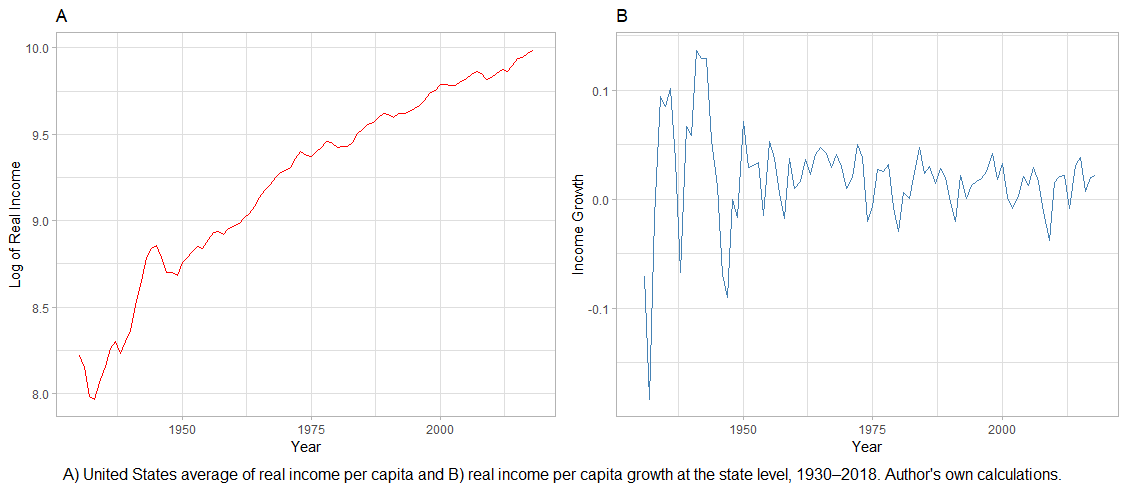
\includegraphics[width=1\linewidth]{images/Fig1_US_Income_gridplot} \caption{\label{Fig1}}\label{fig:Fig1}
\end{figure}

In terms of inequality metrics, Figure {[}\ref{Fig2}{]} gives the
state-average inequality measures from 1930 to 2018, which, again,
replicates the same plot in Atems \& Jones
(\protect\hyperlink{ref-atems}{2015}). However, it is important to note
that the current analysis will emphasize only the Gini-coefficient
(displayed in green), as the robustness checks performed by Atems \&
Jones (\protect\hyperlink{ref-atems}{2015}) with respect to different
measures were deemed adequate for our purposes.

\begin{figure}[H]
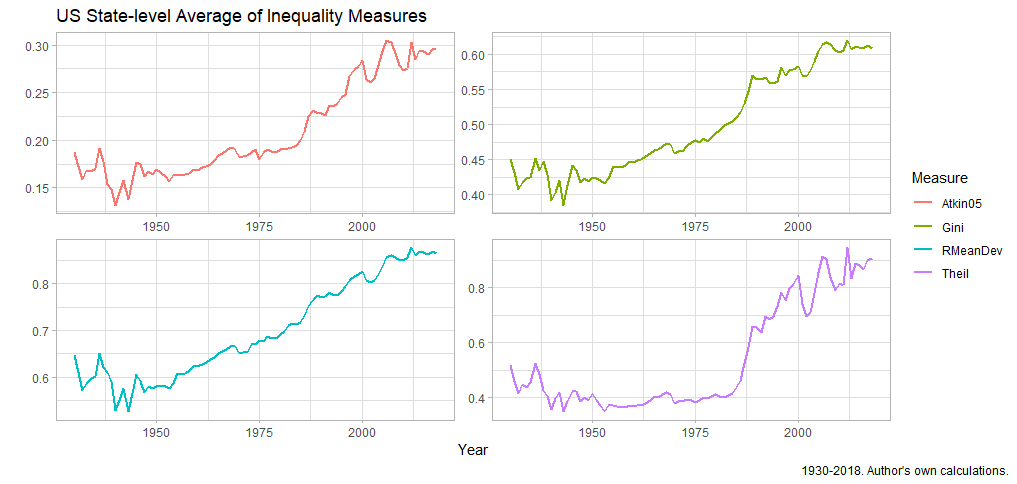
\includegraphics[width=1\linewidth]{images/Fig2_Inequality_Measures} \caption{\label{Fig2}}\label{fig:Fig2}
\end{figure}

\hypertarget{unit-root-tests}{%
\subsection{\texorpdfstring{Unit Root Tests
\label{Section 3.2}}{Unit Root Tests }}\label{unit-root-tests}}

We employ three tests for unit roots\footnote{The Fischer-type ADF, LLC
  and IPS tests. The HT test was excluded as it was not available on the
  statistical program this study employed (the `\emph{plm}' package from
  Croissant \emph{et al.}
  (\protect\hyperlink{ref-croissant2020package}{2020})).}, and one
explicitly for stationarity\footnote{The Hadri LM test.}. Like Atems \&
Jones (\protect\hyperlink{ref-atems}{2015}), these tests are performed
on demeaned data, and the panel data is balanced. Our results are
displayed in the Appendix, section \Ref{A}. Our results, which include
the new data from 2005 to 2018, mirror their findings. Although the
three unit root tests indicate stationarity in levels for both income
per capita and inequality, the Hadri test indicates that the null of no
unit roots cannot be rejected for the series of both variables. All
tests indicate stationarity in the growth rates of the two variables.

\hypertarget{results-baseline-pvar}{%
\subsection{\texorpdfstring{Results Baseline PVAR
\label{Section 3.3}}{Results Baseline PVAR }}\label{results-baseline-pvar}}

The baseline PVAR estimated in this section will follow the same
methodology described in Atems \& Jones
(\protect\hyperlink{ref-atems}{2015}), using equation \ref{eq2}. The
models are estimated using GMM for four lags, and a Cholesky
decomposition is used to identify the structural error terms. Impulse
response functions are generated accordingly. Our results are displayed
using cumulative orthogonalized IRFs (COIRFs), which, as mentioned
earlier, should be interpreted as long run responses to a permanent
shock in the level of the series.\footnote{All estimation of PVARs, and
  computation of OIRFs, were done using a statistical package in R,
  `\emph{panelvar}', developed recently by Sigmund \& Ferstl
  (\protect\hyperlink{ref-sigmund2019panel}{2019}).}. COIRFs were
computed manually from the OIRFs given in Appendix \ref{B}, which have
been included for completeness, and as an additional
extension.\footnote{They are displayed and briefly interpreted in the
  appendix, as the focus of our findings is on cumulative IRFs, as done
  by Atems \& Jones (\protect\hyperlink{ref-atems}{2015}).}

To test for robustness given new data, we estimate two PVARs. The first
includes only the sample of the annual series from 1930 to 2005, and is
thus an exact replication of the baseline PVAR by Atems \& Jones
(\protect\hyperlink{ref-atems}{2015}). The second model applies the PVAR
methodology to the full dataset, including new data. The intuition
behind this approach is that the baseline model can be considered robust
to new data if the two models display similar results. As an additional
visualization tool, the FEVD for both models are also reported.

Figure \ref{Fig3} displays the replicated COIRFs for the baseline model
for the 1930-2005 sample. It seems largely similar to the results
obtained by Atems \& Jones (\protect\hyperlink{ref-atems}{2015}), but
with some noticeable differences. The most pertinent difference is the
wider confidence intervals difference is the response to Gini given its
own shock,

COIRF full sample:\footnote{All confidence intervals are calculated at
  the 95\% level and are generated by Monte Carlo simulation based on
  100 draws. The low number of draws were chosen due to computational
  limitations.}

\newpage

\begin{figure}[H]

{\centering 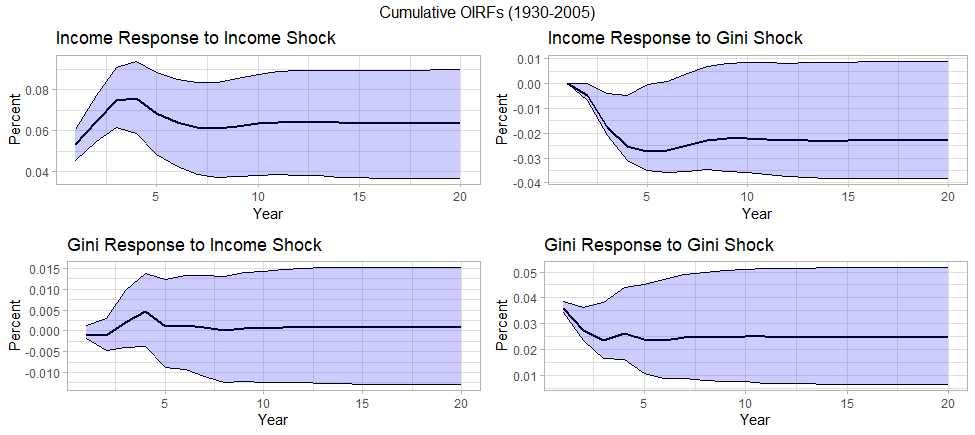
\includegraphics[width=1\linewidth]{images/Fig3_rep_COIRFs} 

}

\caption{\label{Fig3}}\label{fig:Fig3}
\end{figure}

\begin{figure}[H]

{\centering 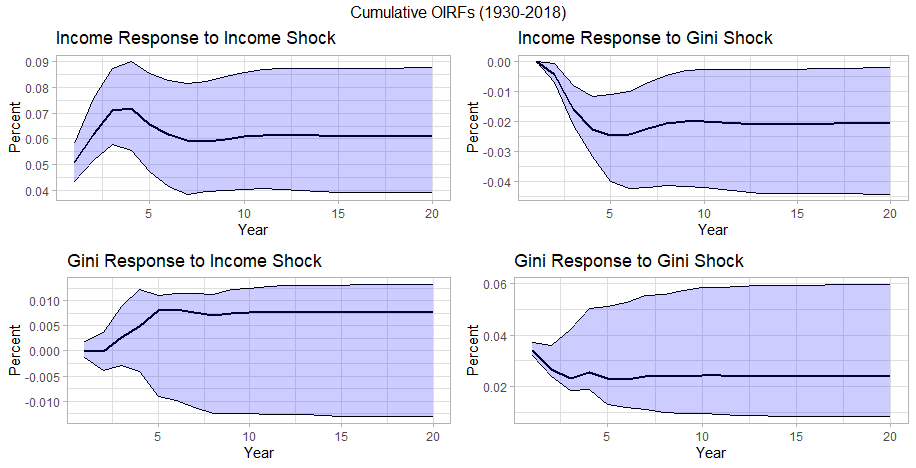
\includegraphics[width=1\linewidth]{images/Fig4_baseline_full_COIRFs} 

}

\caption{\label{Fig4}}\label{fig:Fig4}
\end{figure}

Figure \ref{Fig5} presents the results of the forecast error variance
decompositions for both estimated models. As is evident, they are very
similar, indicating that our model is robust to different sample
periods. For the full-sample model, the variance of Income Growth at
each forecast horizon is explained more by its own shock than for the
replicated (smaller) sample. Conversely, Income Growth variance is thus
also explained less by the shock to inequality. Similarly, Gini Growth
variance

\begin{figure}[H]
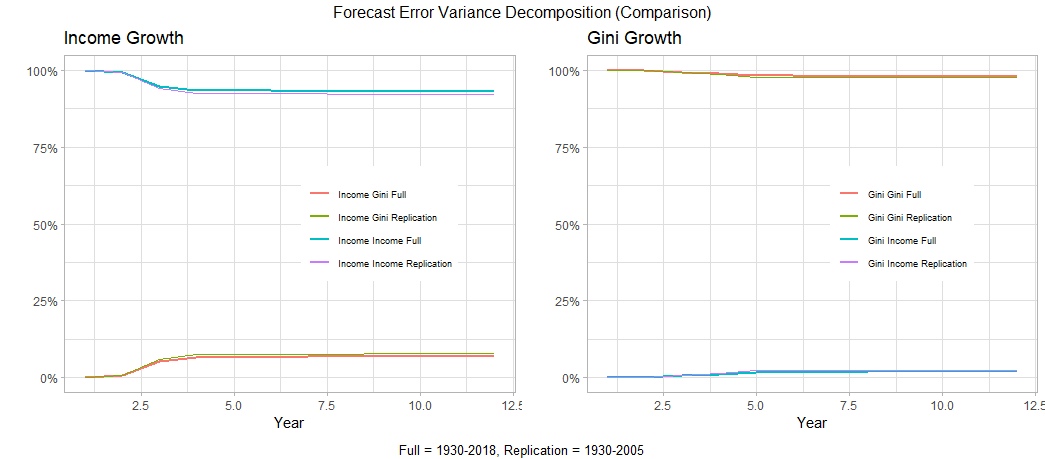
\includegraphics[width=1\linewidth]{images/Fig5_fevd_all} \caption{\label{Fig5}}\label{fig:Fig5}
\end{figure}

\newpage

\hypertarget{regional-subsamples}{%
\subsection{\texorpdfstring{Regional Subsamples
\label{Section 3.4}}{Regional Subsamples }}\label{regional-subsamples}}

In this section, we re-estimate the model for each regional subsample of
the full data. These regions, of which there are eight, are defined
according to geographical area in the US, and are the following:

\hypertarget{conclusion}{%
\section{Conclusion}\label{conclusion}}

\newpage

\hypertarget{references}{%
\section*{References}\label{references}}
\addcontentsline{toc}{section}{References}

\hypertarget{refs}{}
\leavevmode\hypertarget{ref-arellano}{}%
Arellano, M. \& Bover, O. 1995. Another look at the instrumental
variable estimation of error-components models. \emph{Journal of
econometrics}. 68(1):29--51.

\leavevmode\hypertarget{ref-atems}{}%
Atems, B. \& Jones, J. 2015. Income inequality and economic growth: A
panel var approach. \emph{Empirical Economics}. 48(4):1541--1561.

\leavevmode\hypertarget{ref-barro}{}%
Barro, R.J. 2008. \emph{Inequality and growth revisited}. ADB Working
paper series on regional economic integration.

\leavevmode\hypertarget{ref-cingano}{}%
Cingano, F. 2014. Trends in income inequality and its impact on economic
growth.

\leavevmode\hypertarget{ref-croissant2020package}{}%
Croissant, Y., Millo, G., Tappe, K., Toomet, O., Kleiber, C., Zeileis,
A., Henningsen, A., Andronic, L., et al. 2020. Package ``plm''.
\emph{Choice}. 139(1):227--240.

\leavevmode\hypertarget{ref-frank}{}%
Frank, M.W. 2009a. Inequality and growth in the united states: Evidence
from a new state-level panel of income inequality measures.
\emph{Economic Inquiry}. 47(1):55--68.

\leavevmode\hypertarget{ref-frankincome}{}%
Frank, M.W. 2009b. Income inequality, human capital, and income growth:
Evidence from a state-level var analysis. \emph{Atlantic Economic
Journal}. 37(2):173--185.

\leavevmode\hypertarget{ref-levin}{}%
Levin, A., Lin, C.-F. \& Chu, C.-S.J. 2002. Unit root tests in panel
data: Asymptotic and finite-sample properties. \emph{Journal of
econometrics}. 108(1):1--24.

\leavevmode\hypertarget{ref-love}{}%
Love, I. \& Zicchino, L. 2006. Financial development and dynamic
investment behavior: Evidence from panel var. \emph{The Quarterly Review
of Economics and Finance}. 46(2):190--210.

\leavevmode\hypertarget{ref-sigmund2019panel}{}%
Sigmund, M. \& Ferstl, R. 2019. Panel vector autoregression in r with
the package panelvar. \emph{The Quarterly Review of Economics and
Finance}.

\newpage

\hypertarget{appendix}{%
\section*{Appendix}\label{appendix}}
\addcontentsline{toc}{section}{Appendix}

\hypertarget{unit-root-test-results}{%
\subsection{\texorpdfstring{Unit Root Test Results
\label{A}}{Unit Root Test Results }}\label{unit-root-test-results}}

\begin{center}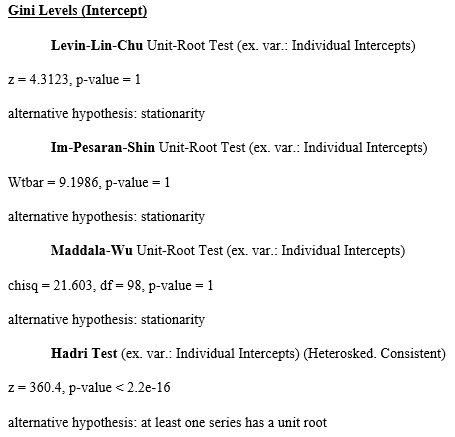
\includegraphics[width=0.49\linewidth,height=0.35\textheight]{images/Gini_Levels_Intercept} 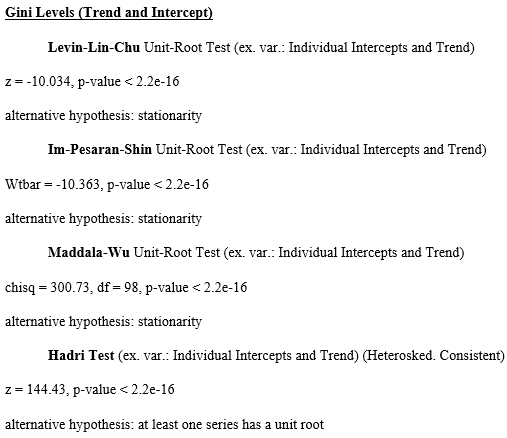
\includegraphics[width=0.49\linewidth,height=0.35\textheight]{images/Gini_Levels_Trend} \end{center}

\begin{center}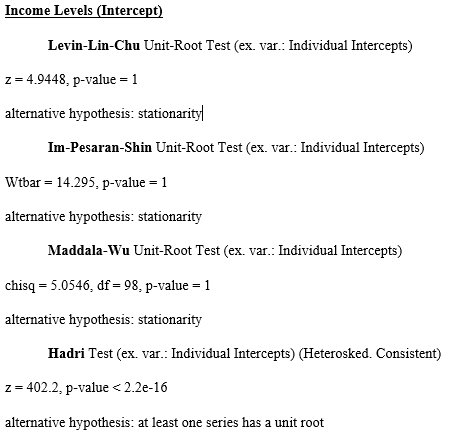
\includegraphics[width=0.49\linewidth,height=0.35\textheight]{images/Income_Levels_Intercept} 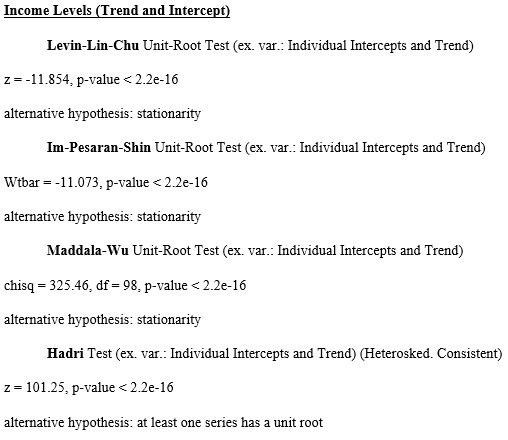
\includegraphics[width=0.49\linewidth,height=0.35\textheight]{images/Income_Levels_Trend} \end{center}

\begin{center}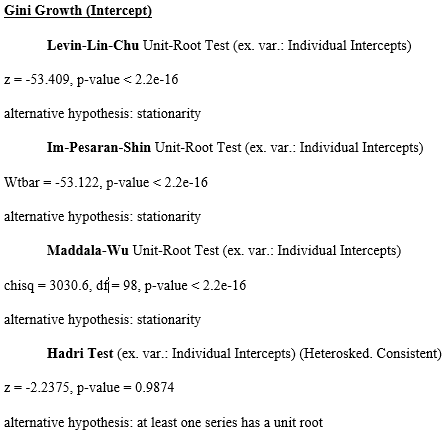
\includegraphics[width=0.49\linewidth,height=0.35\textheight]{images/Gini_Growth_Intercept} 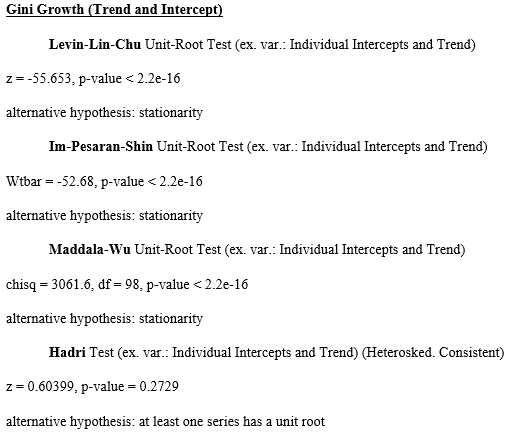
\includegraphics[width=0.49\linewidth,height=0.35\textheight]{images/Gini_Growth_Trend} \end{center}

\begin{center}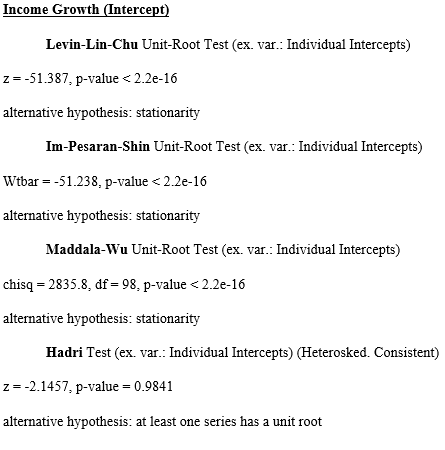
\includegraphics[width=0.49\linewidth,height=0.35\textheight]{images/Income_Growth_Intercept} 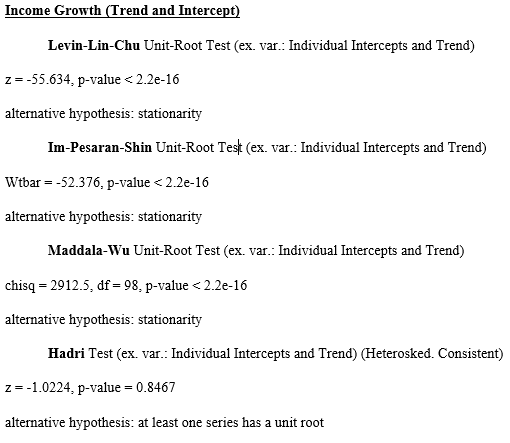
\includegraphics[width=0.49\linewidth,height=0.35\textheight]{images/Income_Growth_Trend} \end{center}

\hypertarget{full-sample-oirfs}{%
\subsection{\texorpdfstring{Full Sample OIRFs
\label{B}}{Full Sample OIRFs }}\label{full-sample-oirfs}}

\begin{figure}[H]
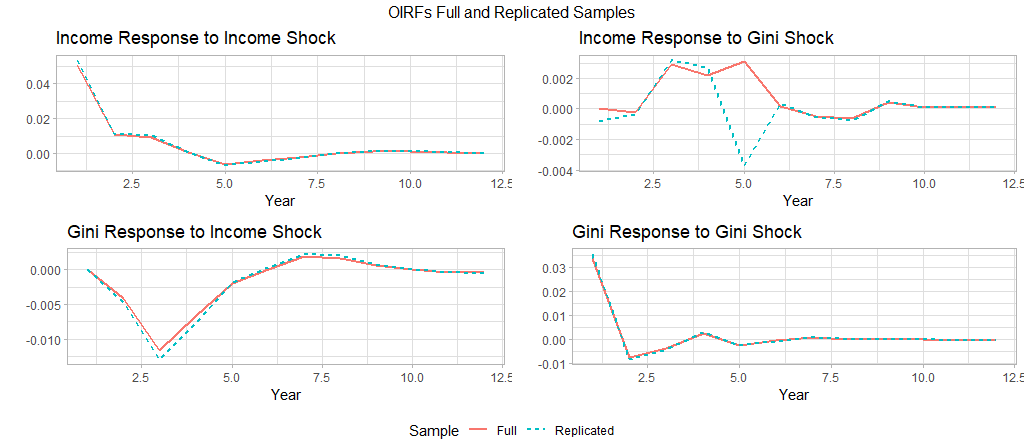
\includegraphics[width=1\linewidth]{images/Appendix_B_OIRFs_both_samples} \caption{\label{Fig6}}\label{fig:AppB}
\end{figure}

\bibliography{Tex/ref}





\end{document}
